\section{Детерминированная коммуникация}

\subsection{Определения}

Для доказательства нижних оценок нам нужны формальные определения.

\begin{definition}
    \deftext{Коммуникационный протокол} для функции $f\colon X \times Y \to Z$~--- это корневое двоичное
    дерево, которое описывает совместное вычисление Алисой и Бобом функции $f$. В этом дереве:
    \begin{itemize}
        \item каждая внутренняя вершина $v$ помечена меткой $a$ или $b$, означающей очередь хода Алисы
            или Боба соответственно;
        \item для каждой вершины, помеченной $a$, определена функция $g_v\colon X \to \{0, 1\}$;
            аналогично, для каждой вершины $v$ с пометкой $b$, определена функция $h_v\colon Y \to \{0,
            1\}$;
        \item каждая внутренняя вершина имеет двух потомков, ребро к первому потомку помечено нулём, а
            ребро ко второму~--- единицей;
        \item каждый лист помечен значением из множества $Z$.
    \end{itemize}

    Пометки $a$ или $b$, означают очередность хода Алисы или Боба соответственно. Функции $g_v$ или $h_v$
    говорят какой бит нужно послать, если вычисление находится в вершине $v$. Таким образом, каждая пара
    входов $(x, y)$ определяет путь от корня до листа в описанном двоичном дереве естественным
    образом. Будем говорить, что коммуникационный протокол \deftext{вычисляет} функцию $f$, если для всех
    пар $(x, y) \in X \times Y $ этот путь заканчивается в листе с пометкой $f(x, y)$.  
    
    \deftext{Коммуникационной сложностью} функции $f$ называется наименьшая глубина протокола,
    вычисляющего функцию $f$. Будем обозначать её символом $\DCC(f)$.
    
    Каждой функции $f$ будем сопоставлять матрицу $M_f$ размера $X \times Y$, в которой в клетке $(x_i,
    y_j)$ стоит значение $f(x_i, y_j)$.
\end{definition}

Следующая лемма нам описывает комбинаторное свойство коммуникационных протоколов, которое нам позволяет
доказывать нижние оценки.

\begin{proposition}
    Рассмотрим дерево протокола со входом из множества $X \times Y$. Рассмотрим в нём произвольную
    вершину $u$. Тогда все входы, из которых можно прийти в вершину $u$, образуют прямоугольник
    $R_u \coloneqq X_u \times Y_u \subseteq X \times Y$.
\end{proposition}

\begin{proof}
    Мы предъявим два способа доказать это утверждение.
    
    \textit{Первый способ:} пусть на входах $(x_1, y_1)$ и $(x_2, y_2)$ мы приходим в вершину $u$. Тогда
    нетрудно убедиться, что на входе $(x_1, y_2)$ Алиса и Боб будут делать те же действия, что и на входах
    $(x_1, y_1)$ и $(x_2, y_2)$ соответственно. Отсюда видно, что входы, приводящие в вершину $u$,
    образуют прямоугольник $R_u = X_u \times Y_u \subseteq X \times Y$. 
    
    \textit{Второй способ:} рассмотрим таблицу элементов $X \times Y$. После первого хода Алисы табличка
    делится пополам горизонтальной линией, так как при одних $x \in X$ Алиса посылает Бобу $1$, а при
    других~--- $0$. Если потом ход делает Боб, то каждый из двух получившихся прямоугольников делится
    своей вертикальной прямой, и так далее. В итоге мы получим разбиение $X \times Y$ на непересекающиеся
    прямоугольники, и каждый из этих прямоугольников соответствует листу в коммуникационном протоколе.  
\end{proof}


Про прямоугольник $R_u$ можно думать в следующим образом: если мы находимся в вершине протокола $u$, то
нам необходимо решить задачу (то есть построить протокол) для всех входов из прямоугольника $R_u$. В
частности этот подход можно рассмотреть, как комбинаторное определение протокола: бинарное дерево, в
котором каждой вершине сопоставлен прямоугольник входов. И если вершины $a, b$ являются потомками $u$, то
$R_u \subseteq R_a \cup R_b$.

Следующая теорема является прямым следствием наших рассуждений про прямоугольники.

\begin{theorem}
    \label{th:rectangle-and-leaves}%
    Пусть для функции $f$ (или отношения) существует коммуникационный протокол с $\ell$ листьями. Тогда
    существует разбиение матрицы $M_f$ на $\ell$ одноцветных комбинаторных прямоугольников.
\end{theorem}

В данной теореме существенно, что мы рассматриваем разбиения, а не любые покрытия, иногда это
важно. Например для $\Search_{\varphi}$, где $\varphi \coloneqq \bigwedge\limits_{i = 1}^{m} C_i$ вся
матрица $M_{\Search_{\varphi}}$ покрывается прямоугольниками вида: $R_i \coloneqq \{(x, y) \mid C_i(x, y)
= 0\}$. Получили всего $m$ прямоугольников. Но маленького разбиения, те не менее, нет.


Эта оценка не всегда точна. Рассмотрим такой пример разбиения таблицы $X \times Y$ на прямоугольники, где в
центре находится прямоугольник из $1$, а вокруг него расположены $4$ прямоугольника из $0$
(см. рис. \ref{fig:partition-rect}). Заметим, что для этого разбиения не существует дерева
протокола. Действительно, рассмотрим первое действие игроков. После него таблица должна поделиться на две
части линией, проходящей через всю таблицу, но такого разреза не существует.
\begin{figure}[h]
 	\centering
    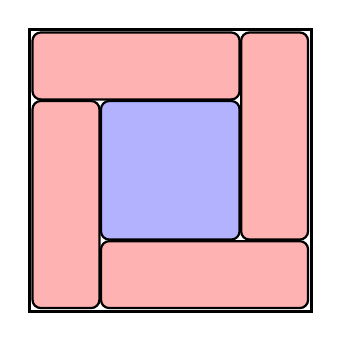
\begin{tikzpicture}[>=latex]
    \def\s{3.5}
    \def\gap{0.85}
    \draw[very thick] (-0.04, -0.04) rectangle (\s + 0.04, \s + 0.04);
    \draw[thick, rounded corners = 3, fill = blue!30] (\gap + 0.02, \gap + 0.02) rectangle
        (\s - \gap - 0.02, \s - \gap - 0.02);
    \draw[thick, rounded corners = 3, fill = red!30] (0, 0) rectangle (\gap, \s - \gap - 0.02);
    \draw[thick, rounded corners = 3, fill = red!30] (0, \s) rectangle (\s - \gap - 0.02, \s - \gap);
    \draw[thick, rounded corners = 3, fill = red!30] (\gap + 0.02, 0) rectangle (\s, \gap);
    \draw[thick, rounded corners = 3, fill = red!30] (\s - \gap, \gap + 0.02) rectangle (\s, \s);
\end{tikzpicture}
 	\caption{}
 	\label{fig:partition-rect}
\end{figure}


Часто в приложениях нас будет интересовать не высота, а размер дерева. Но это все меры связаны.
\begin{theorem}[Балансировка]
    Если существует протокол с $\ell$ листьями, то $\DCC(f) \le 2 \log_{3 / 2} \ell$.
\end{theorem}

\dscomment{переписать}
\begin{proof}
    Берём центроид, проверяем, дойдут ли Алиса и Боб до этой вершины (тратим два бита), спускаемся в один
    из двух кусков.

    В общем, полностью аналогично сведению коммуникации к $\DPLL$.
\end{proof}

Таким образом, если есть нижняя оценка на коммуникационную сложность, то есть нижняя оценка на размер
дерева.

\begin{remark}
    $\DCC(f) \ge \log_2 \ell$, если в любом протоколе для $f$ хотя бы $\ell$ листьев.
\end{remark}


\paragraph{Небалансирующиеся протоколы.}
Другая коммуникация: A и B посылают судье по вещественному числу $a$ и $b$, проверяем, правда ли, что $a
> b$. Идём либо налево, либо направо.

$\GT$ становится тривиальной.

Эта модель слабее вероятностной коммуникации (в вероятностной можно симулировать $\GT$).
Однако, у нас нет нижних оценок на размер (не высоту) протокола!

Не балансируется: есть примеры, когда протокол~--- дерево маленького размера, но высота нужна большая.

\subsection{Нижняя оценка на \texorpdfstring{$\DCC(\EQ)$}{D(EQ)} и \texorpdfstring{$\DCC(\GT)$}{D(GT)}}

\begin{theorem}
    $\DCC(\EQ) = n + 1$.
\end{theorem}

\begin{proof}
    Свойство комбинаторного прямоугольника: $(x, y), (x', y') \in R \implies\allowbreak (x', y), (x,
    y')\in R$.

    $M_{\EQ}$~--- единичная матрица. Две единицы на диагонали не могут быть в одном
    прямоугольнике. Значит, хотя бы $2^n + 1$ прямоугольников. Значит, $\DCC \ge n + 1$.
\end{proof}


\begin{theorem}
    $\DCC(\GT) = n + 1$.
\end{theorem}

\begin{proof}
    Аналогично доказательству для $\EQ$.
\end{proof}


\subsection{Связь протоколов и разбиений/покрытий}

\begin{definition}
    $\chi_0(f)$~--- количество нулевых прямоугольников в минимальном разбиении $M_f$.

    $\chi_1(f)$~--- количество единичных прямоугольников в минимальном разбиении $M_f$.

    $\chi(f) \coloneqq  \chi_0(f) + \chi_1(f)$.
\end{definition}

\begin{definition}
    $C^0(f)$~--- количество нулевых прямоугольников в минимальном покрытии $M_f$.

    $C^1(f)$~--- количество единичных прямоугольников в минимальном покрытии $M_f$.
\end{definition}

Частичное решение проблемы~\ref{itm:problem partition-to-protocol}:
\begin{theorem}
    \label{D < log C0 * log C1}

    Пусть $f$~--- функция (не отношение).

    Тогда для разбиений выполняется:
    $\log \chi \le \DCC(f) \le \bigO{\log \chi_0 \log \chi_1} = \bigO{\log^2 \chi}$.

    И для покрытий выполняется:
    $\log (C^0 + C^1) \le \DCC(f) \le \bigO{\log C^0 \log C^1}$.

    Таким образом, $\log \chi \le \DCC(f) \le \bigO{\log C^0 \log C^1}$.
\end{theorem}


\begin{proof}
    Оценки снизу уже доказывали. Докажем оценки сверху.

    Рассмотрим два любых прямоугольника разбиения: $R' = X' \times Y'$ и $R'' = X'' \times Y''$. Либо
    иксы, либо игреки не пересекаются~--- иначе пересекаются $R'$ и $R''$.

    Алиса и Боб пытаются доказать, что ответ равен 1. Изначально у нас есть все нулевые прямоугольники.

    \begin{enumerate}
        \item Алиса ищет такой $1$-прямоугольник, который содержит её $x$, и при этом запрещающий хотя бы
            половину нулевых прямоугольников (то есть не пересекающийся с ними по координате $X$). Если
            такой есть, посылает Бобу его номер.
        \item Иначе Боб делает то же самое, пытаясь уменьшить хотя бы вдвое количество потенциальных
            нулевых прямоугольников.
        \item Если нулевые прямоугольники закончились, то ответ единица. Если не закончились, то
            утверждаем, что ответ ноль.
    \end{enumerate}

    От противного, посмотрим на 1-прямоугольник, в котором лежит $(x, y)$. Этот прямоугольник
    пересекается по $X$ более чем с половиной 0-прямоугольников, и по $Y$ более чем с половиной
    0-прямоугольников. Но тогда есть 0-прямоугольник, с которым он пересекается и по $X$, и по $Y$,
    значит, у них есть общая точка. Противоречие.

    Раундов $\ceil{\log \chi_0}$, в каждом пересылаем $\ceil{\log \chi_1}$ бит.

    Отметим, что мы не пользовались тем, что у нас разбиение, а не покрытие. Но пользовались тем, что
    дана функция, а не отношение, то есть ответ однозначен.
\end{proof}